\documentclass[12pt,a4paper]{article}
\usepackage[utf8]{inputenc}
\usepackage[T1]{fontenc}
\usepackage[margin=2.5cm]{geometry}
\usepackage{hyperref}
\usepackage{enumitem}
\usepackage{tabularx}
\usepackage{booktabs}
\usepackage{float}
\usepackage{graphicx}

\title{\textbf{EduRAG - Asynchronous AI Knowledge Base} \\ \large Milestone 1: Architecture, Storage Logic \& Terraform Presentation}
\author{Anna Ostrowska, Michał Kukla, Norbert Frydrysiak}
\date{\today}

\begin{document}

\maketitle

\section{Brief Description}
EduRAG is a highly scalable, AI-powered knowledge base utilizing the Retrieval-Augmented Generation (RAG) architecture. The platform allows users to upload massive volumes of textual data, such as gigabytes of textbooks, manuals, or research papers. To ensure a large-scale assumption, the system decouples the responsive user interface from the data processing layer. 

By leveraging a Serverless/PaaS event-driven architecture heavily based on Google Cloud Platform (GCP) and Firebase, uploaded documents are asynchronously read, chunked, and converted into embeddings in the background. Once processed, end-users can "chat" with the uploaded documents via a responsive UI, while the system dynamically retrieves the most relevant context to answer their queries using Google's Vertex AI models.

\section{Main Features}
\begin{itemize}[label=\textbullet]
    \item \textbf{Asynchronous Document Ingestion Pipeline:} Direct-to-storage uploads to Google Cloud Storage trigger Pub/Sub event queues. Serverless background workers (Cloud Run / Cloud Functions) consume these events to perform heavy PDF parsing, text chunking, and embedding generation without blocking the frontend.
    \item \textbf{Interactive Chat UI:} A fast, lightweight web interface hosted on Firebase Hosting where users can ask questions in natural language. The UI connects to a serverless API that performs similarity searches and streams LLM-generated answers.
    \item \textbf{Scalable Vector Storage \& Metadata:} The generated text embeddings are stored in a Vector Database (e.g., Vertex AI Vector Search or ChromaDB on Cloud Run) optimized for semantic search. Transactional metadata and chat histories are stored in Firestore.
    \item \textbf{Real-Time Processing Status:} Users uploading large datasets can monitor the progress of the vectorization jobs via the dashboard, synchronized in real-time via Firestore listeners.
    \item \textbf{Infrastructure as Code (IaC):} All cloud resources, including storage buckets, serverless functions, message queues, and databases, are fully provisioned and managed using Terraform (Google Provider).
\end{itemize}

\section{System Architecture \& Microservices Strategy}
To fulfill the serverless and PaaS requirements, the system is built entirely on GCP. The architecture is strictly divided into two decoupled workflows to ensure high availability and responsiveness:

\subsection{Workflow 1: Asynchronous Ingestion Pipeline (Heavy Load)}
\begin{enumerate}
    \item \textbf{Direct Upload:} The frontend requests a pre-signed URL from the API and uploads a large PDF directly to Google Cloud Storage (GCS), completely bypassing the backend compute servers.
    \item \textbf{Event Trigger:} A successful upload to GCS triggers an Eventarc notification, which drops a message into a Google Cloud Pub/Sub topic.
    \item \textbf{Background Processing:} A Cloud Run service consumes the Pub/Sub message, downloads the PDF from GCS, and uses LangChain to split the text into smaller, overlapping chunks.
    \item \textbf{Vectorization \& Storage:} The worker calls the Vertex AI Embeddings API to convert text chunks into vectors, which are then upserted into the Vector Database.
\end{enumerate}

To further illustrate the event-driven nature of the platform, Figure \ref{fig:sequence} details the exact step-by-step system interactions during the heavy document upload and vectorization process.

\begin{figure}[H]
    \centering
    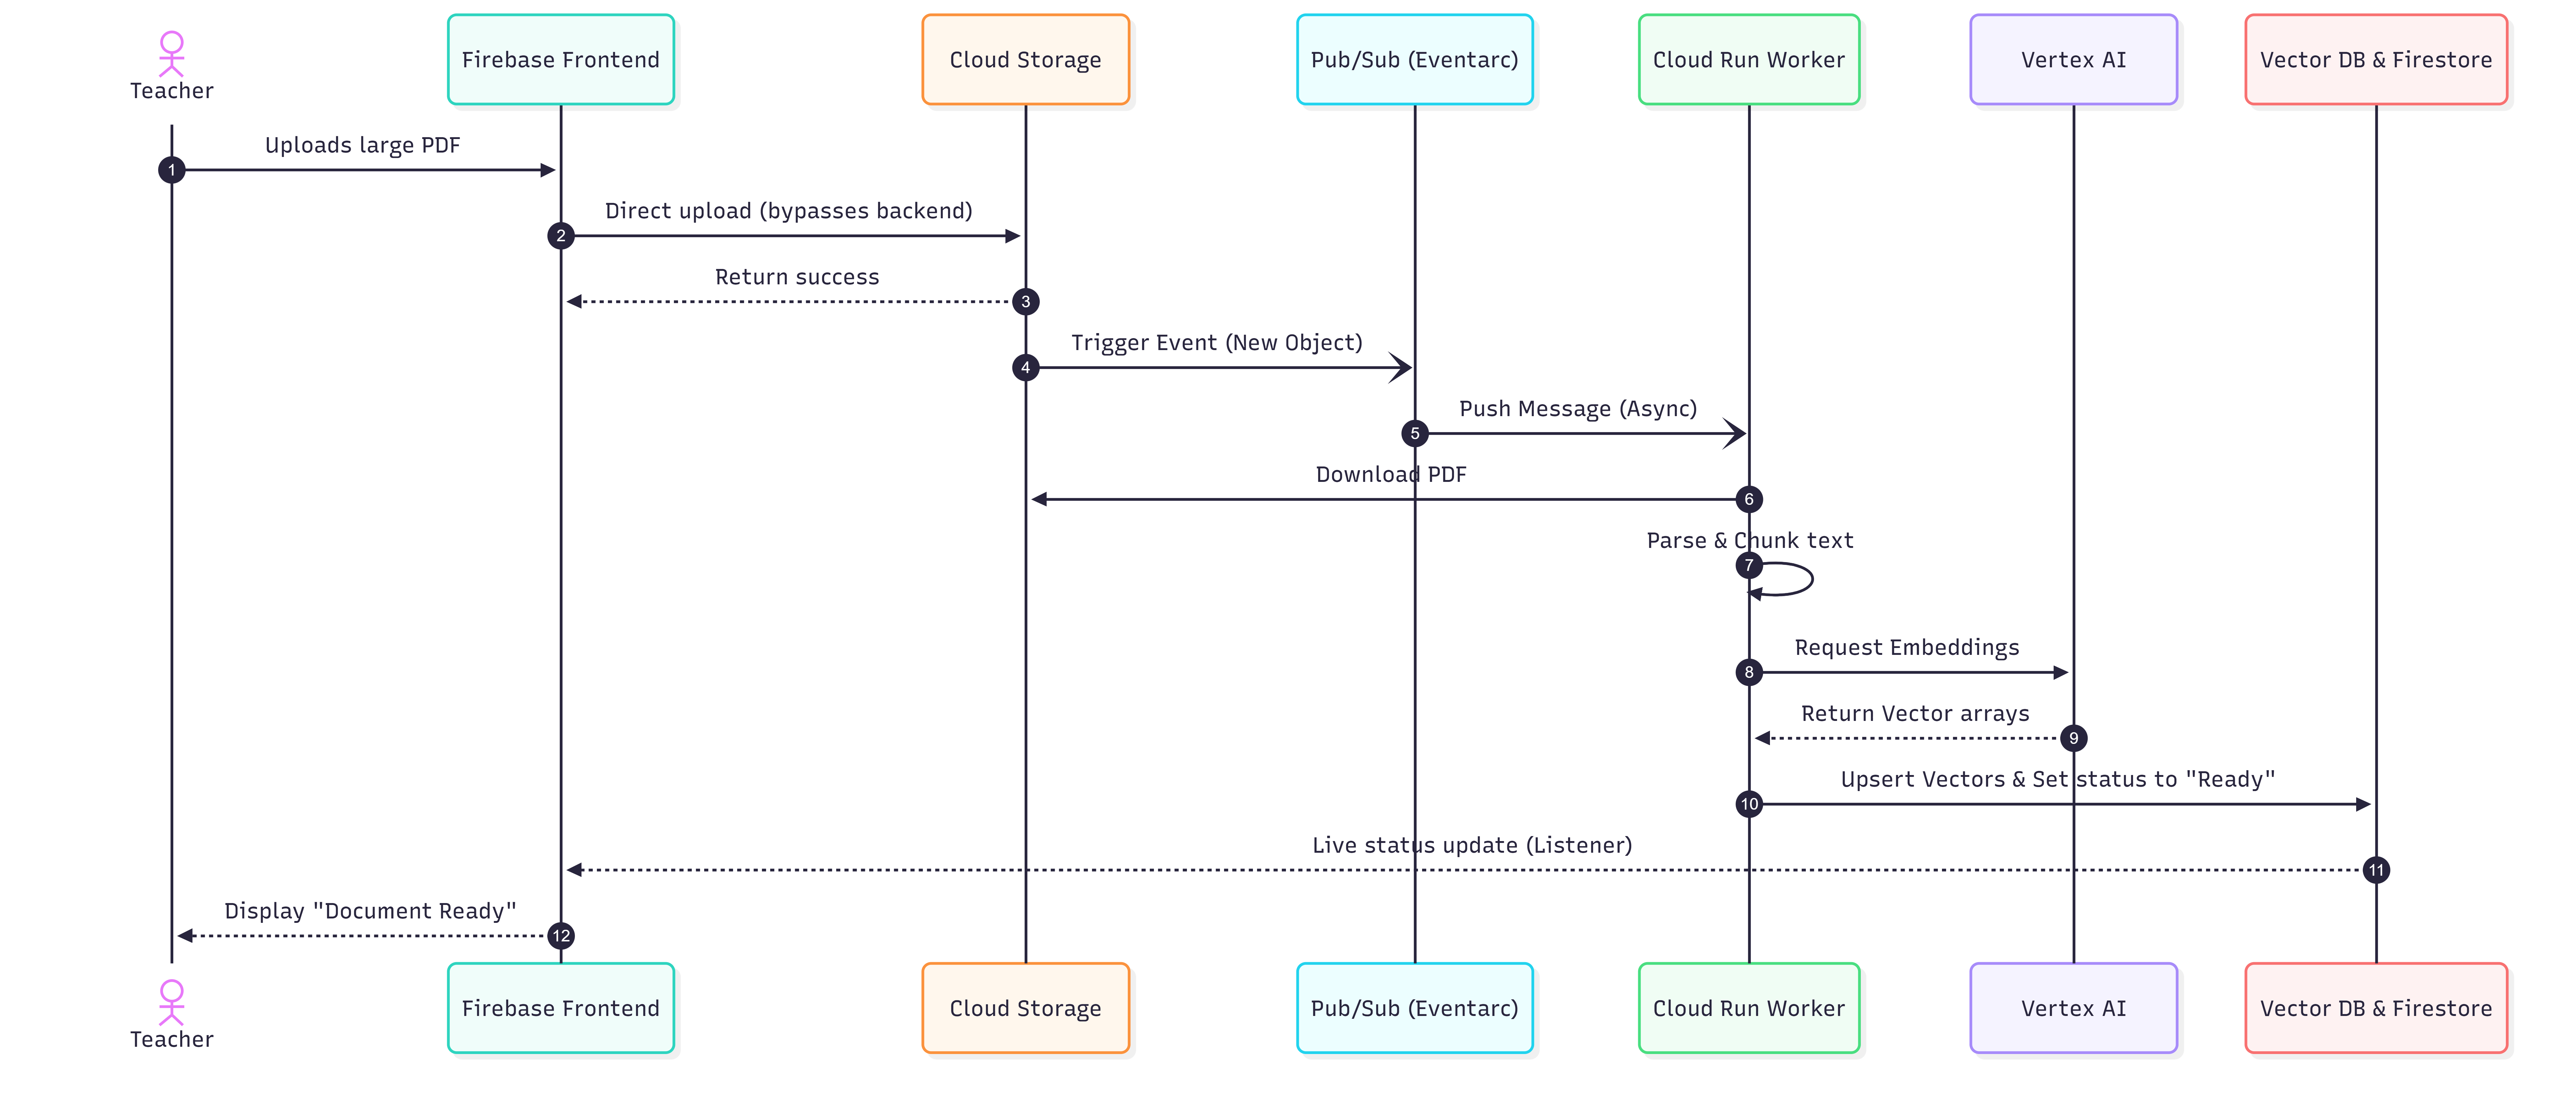
\includegraphics[width=0.95\linewidth]{sequence.png}
    \caption{Sequence diagram illustrating the asynchronous document ingestion pipeline.}
    \label{fig:sequence}
\end{figure}
\subsection{Workflow 2: Real-time Inference Pipeline (Low Latency)}
\begin{enumerate}
    \item \textbf{Querying:} The user types a question in the UI. The request is routed via an API Gateway to a lightweight Cloud Function.
    \item \textbf{Similarity Search:} The function converts the user's question into a vector (via Vertex AI) and queries the Vector DB for the top-K most semantically similar text chunks.
    \item \textbf{LLM Generation:} The retrieved chunks are injected into a prompt as context. The Gemini model (via Vertex AI) generates a final response based strictly on the provided context, which is streamed back to the UI.
\end{enumerate}
The following architecture diagram (Figure \ref{fig:architecture}) provides a comprehensive overview of the EduRAG ecosystem. It illustrates the decoupling between the high-load ingestion process and the low-latency user interaction layer. The red arrows represent the asynchronous data flow for document processing, while the blue arrows delineate the real-time inference path for the chat interface:
\begin{figure}[H]
    \centering
    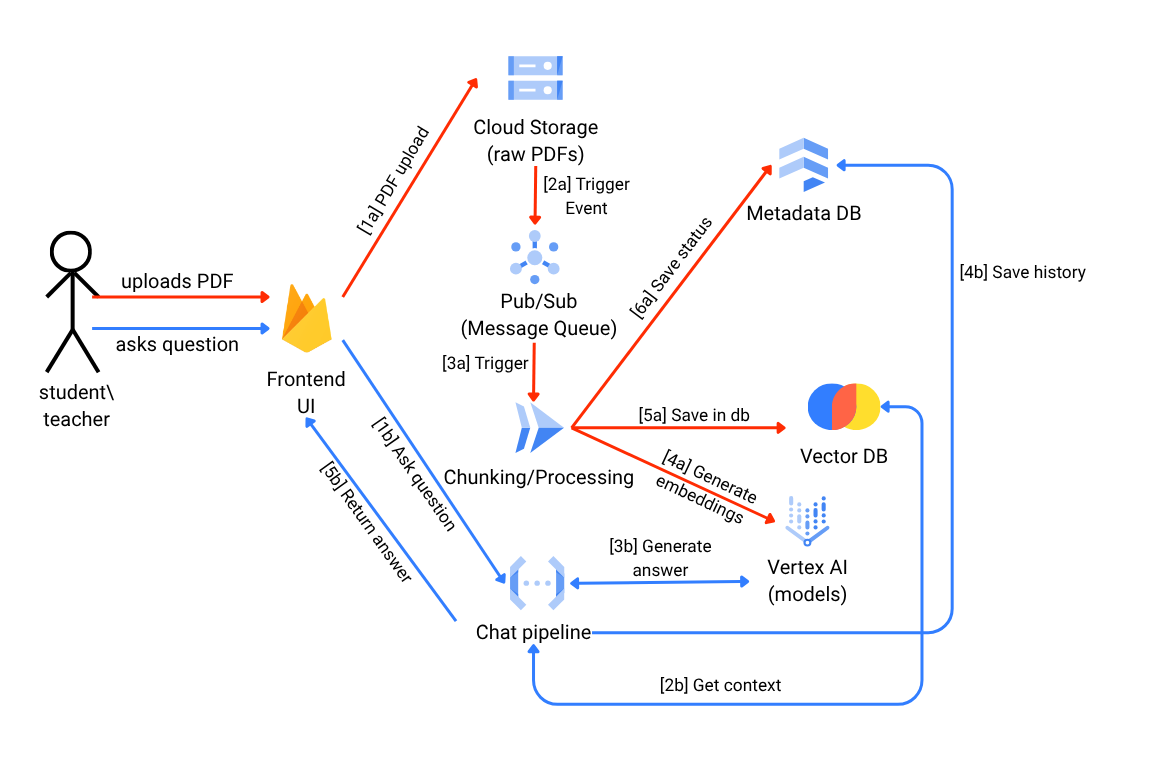
\includegraphics[width=1\linewidth]{architecture.png}
    \caption{High-level system architecture of EduRAG on Google Cloud Platform, with decoupled ingestion (red) and inference (blue) pipelines.}
    \label{fig:architecture}
\end{figure}
\section{Storage Characteristics}
The system utilizes a multi-tiered storage strategy to optimize costs and performance, tailored to specific data types and access patterns:
\begin{itemize}[label=\textbullet]
    \item \textbf{Google Cloud Storage (GCS):}
    \begin{itemize}
        \item \textit{Type:} Unstructured (Raw PDF files).
        \item \textit{Architecture:} Object Storage.
        \item \textit{Consistency:} Strong Consistency.
        \item \textit{Amount of Data:} High (Gigabytes/Terabytes of textbooks).
        \item \textit{Access Pattern:} Write-Once, Read-Rarely (read only once by the worker during the chunking phase).
    \end{itemize}
    \item \textbf{Firestore (Metadata DB):}
    \begin{itemize}
        \item \textit{Type:} Structured / Semi-structured (JSON profiles, job statuses).
        \item \textit{Architecture:} NoSQL Document Database.
        \item \textit{Consistency:} Strong Consistency (for document lookups).
        \item \textit{Amount of Data:} Low / Medium (Megabytes).
        \item \textit{Access Pattern:} High Read \& Write (frequent updates of background job statuses synchronized to the UI).
    \end{itemize}
    \item \textbf{Vector Database (Vertex AI / ChromaDB):}
    \begin{itemize}
        \item \textit{Type:} Structured (Float arrays / Embeddings).
        \item \textit{Architecture:} NoSQL Vector Index.
        \item \textit{Consistency:} Eventual Consistency.
        \item \textit{Amount of Data:} Medium / High.
        \item \textit{Access Pattern:} Write-Once, Read-Many (constant read requests from the Chat API).
    \end{itemize}
\end{itemize}
\section{Design APIs (REST Contracts)}
The system decouples heavy processing from the user interface using lightweight RESTful API endpoints exposed via Cloud Run.
\begin{itemize}[label=\textbullet]
    \item \textbf{Generate Upload URL (GET /api/v1/documents/upload-url):} Generates a pre-signed Google Cloud Storage URL. It allows the frontend to upload large PDFs directly to the bucket, receiving a JSON with the \texttt{upload\_url} and a unique \texttt{document\_id}.
    \item \textbf{Chat / Inference Endpoint (POST /api/v1/chat):} Accepts a user query via JSON containing \texttt{document\_id} and the \texttt{query} string. It performs a similarity search in the Vector DB and returns the LLM-generated \texttt{answer} along with \texttt{retrieved\_context\_sources}.
\end{itemize}

\section{Reliability Metrics (SLA, SLO, SLI)}
To ensure high availability and responsiveness of the knowledge base, the following reliability metrics are defined:
\begin{itemize}[label=\textbullet]
    \item \textbf{SLA (Service Level Agreement):} The platform guarantees a 99.9\% uptime for the Chat UI and Inference API, backed by GCP's managed services availability.
    \item \textbf{SLO (Service Level Objectives):}
    \begin{itemize}
        \item \textit{Real-time Inference:} 95\% of all \texttt{/api/chat} requests will return an LLM-generated response in under 4 seconds.
        \item \textit{Asynchronous Ingestion:} 99\% of all uploaded PDF documents (under 50 MB) will be fully parsed, chunked, vectorized, and ready for querying within 3 minutes of upload.
    \end{itemize}
    \item \textbf{SLI (Service Level Indicators):}
    \begin{itemize}
        \item \textit{Inference Latency:} The average execution time of the Cloud Run API handling the chat endpoint.
        \item \textit{Ingestion Processing Time:} The time delta between the document upload timestamp in Firestore and the "Ready" status update.
    \end{itemize}
\end{itemize}
\section{Team Roles \& Responsibilities (Cloud Domains)}
To ensure every team member engages with cloud technologies, the workload is divided by \textbf{Cloud Domains}. Every member is responsible for writing the Terraform configuration for their respective cloud resources.

\begin{enumerate}
    \item \textbf{Cloud Storage \& Edge Architect:} Responsible for the cloud entry points. Manages the deployment of the Chat UI via Firebase Hosting, configures Google Cloud Storage with CORS and signed URLs for secure direct-to-cloud document uploads, and writes the associated Terraform scripts.
    \item \textbf{Asynchronous Compute \& Messaging Engineer:} Focuses on the event-driven core. Responsible for provisioning Pub/Sub Message Queues, configuring Eventarc Triggers, deploying the Cloud Run Background Workers that chunk the PDFs, and writing the associated Terraform scripts.
    \item \textbf{Cloud Data \& ML Integration Lead:} Manages data persistence and AI services. Responsible for provisioning the Vector Database, configuring Firestore collections for background job metadata, integrating Vertex AI (Gemini and Embeddings), and writing the associated Terraform scripts including IAM Service Accounts.
\end{enumerate}

\section{Project Schedule}
The project follows the official course milestones. For Milestone 1, the core infrastructure design and initial Terraform configurations have been completed.

\vspace{0.5cm}
\noindent
\begin{tabularx}{\textwidth}{@{} l l X @{}}
\toprule
\textbf{Date} & \textbf{Phase} & \textbf{Tasks \& Milestones} \\
\midrule
Apr 17, 2026 & M0 & \textbf{Project Submission:} Document outlining project idea. (Completed) \\
\addlinespace
Apr 18 -- 26 & Design & Draw microservices diagram, define API contracts, and draft initial Terraform configurations for GCP. \\
\addlinespace
\textbf{May 08, 2026} & \textbf{M1} & \textbf{Document \& Plan Presentation:} Present updated GCP microservices, storage logic, and working Terraform. \\
\addlinespace
May 08 -- 22 & Build & Develop Serverless workers (Cloud Run), integrate Vertex AI API, connect Firebase Frontend, and test Pub/Sub. \\
\addlinespace
May 23 -- Jun 02 & Scale Test & Perform load testing with massive PDFs to validate the "large scale assumption" and tune GCS/Pub/Sub limits. \\
\addlinespace
\textbf{Jun 03, 2026} & \textbf{M2} & \textbf{Final Presentation:} Live demo of the asynchronous uploading and real-time chat processing. \\
\bottomrule
\end{tabularx}

\end{document}